\section{Fluxionnal compiler} \label{section:compiler}

The source languages we focus on should offer higher-order functions and be implemented as an event-loop with a global memory.
Javascript is such a language and is often implemented on top of an event-loop, like in \textit{Node.js}.
We developed a compiler that transforms a \textit{Node.js} application into a fluxional application compliant with the execution model described in section \ref{section:model}.
Our compiler uses the \textit{estools}\ftnt{https://github.com/estools} suite to parse, manipulate and generate source code from Abstract Syntax Tree (AST).
And it is tailored for -- but not limited to -- web applications using \textit{Express}\ftnt{http://expressjs.com/}, the most used \textit{Node.js} web framework.

\begin{figure}
  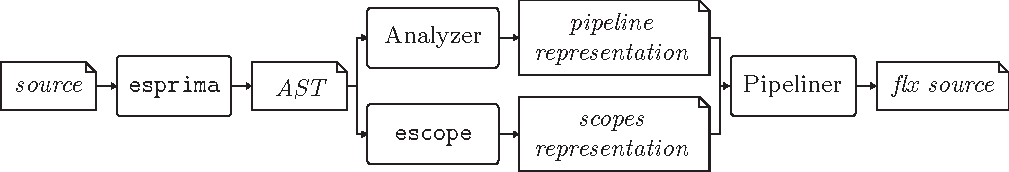
\includegraphics[width=\linewidth]{compiler-stream.pdf}
  \caption{Compilation chain}
  \label{fig:compilation}
\end{figure}

The chain of compilation is described in figure \ref{fig:compilation}.
The compiler extracts an AST from the source with \texttt{esprima}.
From this AST, the \textit{Analyzer} step identifies the limits of the different application parts and how they relate to form a pipeline.
This first step outputs a pipeline representation of the application.
Section \ref{section:compiler:analyzer} explains this first compilation step.
In the pipeline representation, the stages are not yet independent and encapsulated into fluxions.
From the AST, \texttt{escope} produces a representation of the memory scopes.
The \textit{Pipeliner} step analyzes the pipeline representation and the scopes representation to distribute the shared memory into independent groups of fluxions.
Section \ref{section:compiler:pipeliner} explains this second compilation step.

\subsection{Analyzer step} \label{section:compiler:analyzer}

The limit between two application parts is defined by a rupture point.
The analyzer identifies these rupture points, and outputs a representation of the application in a pipeline form.
Application parts are the stages, and rupture points are the message streams of this pipeline.

\subsubsection{Rupture points} \label{section:compiler:analyzer:rupture}

A rupture point is a call of a loosely coupled function.
It is an asynchronous call without subsequent synchronization with the caller.
In \textit{Node.js}, I/O operations are asynchronous functions and indicate rupture points between two application parts.
Figure \ref{fig:basicrp} shows a code example of a rupture point with the illustration of the execution of the two application parts isolated into fluxions.
The two application parts are the caller of the asynchronous function call on one hand, and the callback provided to the asynchronous function call on the other hand.

\begin{figure}[h!]
  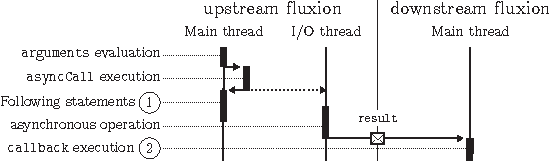
\includegraphics[width=\linewidth]{basicrp.pdf}
  \begin{code}
asyncCall(arguments, function callback(result){ //@\circled{2}@ });
// Following statements //@\circled{1}@
  \end{code}
  \caption{Rupture point interface}
  \label{fig:basicrp}
\end{figure}

A callback is a function passed as a parameter to a function call.
It is invoked by the callee to continue the execution with data not available in the caller context.
There are three kinds of callbacks, but only two are asynchronous: listeners and continuations.
The two corresponding types of rupture points are \textit{start} and \textit{post}.

\textbf{Start rupture points} (listeners) are on the border between the application and the outside, continuously receiving incoming user requests.
An example of a start rupture point is in listing \ref{lst:source}, between the call to \texttt{app.get()}, and its listener \texttt{handler}.
These rupture points indicate the input of a data stream in the program, and the beginning of a chain of fluxions to process this stream.

\textbf{Post rupture points} (continuations) represent a continuity in the execution flow after an asynchronous operation yielding a unique result, such as reading a file, or a database.
An example of a post rupture points is in listing \ref{lst:source}, between the call to \texttt{fs.readFile()}, and its continuation \texttt{reply}.

\subsubsection{Detection}

The compiler uses a list of common asynchronous callees, like the \texttt{express} and file system methods.
This list can be augmented to match asynchronous callees individually for any application.
To identify the callee, the analyzer walks the AST to find a call expression matching this list.

After the identification of the callee, the callback needs to be identified as well, to be encapsulated in the downstream fluxion.
For each asynchronous call detected, the compiler tests if one of the arguments is of type \texttt{function}.
Some callback functions are declared \textit{in situ}, and are trivially detected.
For variable identifiers, and other expressions, the analyzer tries to detect their type.
The analyzer walks back the AST to track their assignations and modifications, so as to determine their last value.

\subsection{Pipeliner step} \label{section:compiler:pipeliner}

A rupture point eventually breaks the chain of scopes between the upstream and downstream fluxion.
The closure in the downstream fluxion cannot access the scope in the upstream fluxion as expected.
The pipeliner step replaces the need for this closure, allowing application parts to rely only on independent memory stores and message passing.
It determines the distribution using the scope representation, which represents the variables' dependencies between application parts.
Depending on this representation, the compiler can replace the broken closures in three different ways.
We present these three alternatives in figure \ref{fig:states}.

\begin{figure}[h!]
  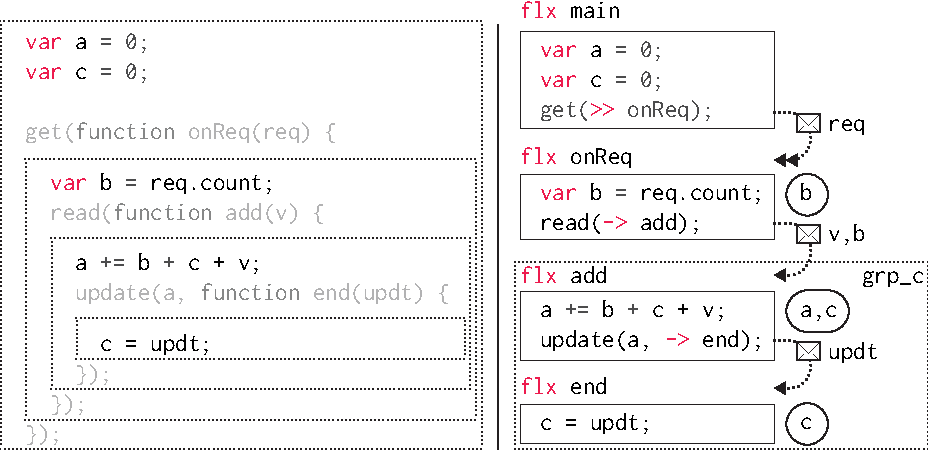
\includegraphics[width=\linewidth]{states.pdf}
  \caption{Variable management from Javascript to the high-level fluxionnal language}
  \label{fig:states}
\end{figure}

\paragraph{Scope}
If a variable is modified inside only one application part in the current \textit{post} chain, then the pipeliner adds it to the context of its fluxion.

In figure \ref{fig:states}, the variable \texttt{a} is updated in the function \texttt{add}.
The pipeliner step stores this variable in the context of the fluxion \texttt{add}.

\paragraph{Stream}
If a modified variable is read by downstream application parts, then the pipeliner makes the upstream fluxion add this variable to the message stream to be sent to the downstream fluxions.
It is impossible to send variables to upstream flux\-ions, without causing inconsistencies.
If the fluxion retro propagates the variable for an upstream fluxion to read, the upstream fluxion might use the old version while the new version is on its way.

In figure \ref{fig:states}, the variable \texttt{b} is set in the function \texttt{onReq}, and read in the function \texttt{add}.
The pipeliner step makes the fluxion \texttt{onReq} send the updated variable \texttt{b}, in addition to the variable \texttt{v}, in the message sent to the fluxion \texttt{add}.

Exceptionally, if a variable is defined inside a \textit{post} chain, like \texttt{b}, then this variable can be streamed inside this \textit{post} chain without restriction on the order of modification and read.
Indeed, the execution of the upstream fluxion for the current \textit{post} chain is assured to end before the execution of the downstream fluxion.
Therefore, no reading of the variable by the upstream fluxion happens after the modification by the downstream fluxion.

\paragraph{Share}
If a variable is needed for modification by several application parts, or is read by an upstream application part, then it needs to be synchronized between the fluxions.
To respect the semantics of the source application, we cannot tolerate inconsistencies.
Therefore, the pipeliner groups all the fluxions sharing this variable with the same tag.
And it adds this variable to the contexts of each fluxions.

In figure \ref{fig:states}, the variable \texttt{c} is set in the function \texttt{end}, and read in the function \texttt{add}.
As the fluxion \texttt{add} is upstream of \texttt{end}, the pipeliner step groups the fluxion \texttt{add} and \texttt{end} with the tag \texttt{grp\_c} to allow the two fluxions to share this variable.